% vim: set foldmethod=marker : %

% Hearing Faith: Music as Theology in the Spanish Empire
% 
% Andrew A. Cashner
% 
% Chapter 4, Heavenly Dissonance
% (Cererols, *Suspended, cielos*)
%
% 2015-03     Dissertation defended
% 2018-04-13  New version begun for book
% 2018-05-22  Converted to LaTeX
% 2018-06-12  New version resumed
% 2018-10-01  Continued by hand
% 2019-03-04  Type MS
% 2019-04-18  Complete typing MS and fill in genealogy, poetry
% 2019-09-09  Revising after whole book draft completed
% 2019-09-16  Add section and bibliography on astrology, science
% 2020-02-10  Final revisions

\chapter{Heavenly Dissonance (Montserrat, 1660s)}
\label{ch:cererols-suspended}

\epigraph
{Suspended, cielos, vuestro dulce canto. \\
Tened, parad, y escuchad \\
la más nueva consonancia \\
que forman en su distancia \\
lo eterno y lo temporal}
{Anonymous, \wtitle{Suspended, cielos} (Montserrat, \circa{1660})}

%{{{1 intro
Pilgrims who reached the mountaintop Abbey of Our Lady of Montserrat in time for
Christmas services were primed for experiences of exaltation.
Perched on a jagged peak overlooking the Barcelona region, the abbey church
enshrined the statue of the Black Virgin of Montserrat, patron of Catalonia.
Many came in search of miracles or in payment of spiritual debts, and though
they came to see the Virgin, they also came to hear the abbey's famous school
choir, the Escolania---today the oldest continuously operating singing school in
the world.%
    \Autocite
    [On Spanish Marian devotion and shrines, see][]
    {Christian:LocalReligion}
This was the environment in which the villancico by Joan Cererols,
\wtitle{Suspended, cielos, vuestro dulce canto}, was first heard.%
\begin{Footnote}
    \sig{E-CAN}{AU 0116}, 
    \autocites
    [35--36, 49--118]{Cashner:WLSCM32}
    [xxv, 221--236]{Cererols:MEM-VC}.
\end{Footnote}
The chorus addressed the celestial spheres themselves, commanding them to cease
their perpetual music and listen.  
A new song, \quoted{the newest consonance}, was forming in the person of the
Christ-child. 
As \term{Verbum infans} his cries would form the basis for the music of a
renewed creation.
By the end of the piece, attentive listeners could actually hear the theme
representing Christ's voice become the \term{cantus firmus} of a new heavenly
music. 
The piece was a school for spiritual listening within a Neoplatonic tradition:
it challenged hearers to listen beyond this depiction of heavenly music for the
higher, unhearable music of Christ himself.


\index{listening!for higher music}
\index{Cererols, Joan|(}
\index{Montserrat!Abadia|(}
\index{Montserrat!Escolania}
\index{music of the spheres}
\index{cosmos}
\index{\emph{Verbum infans}}
\index{sanctoral devotion!Mary}

The setting by Cererols is one of ten known versions of this villancico,
performed between 1650 and 1700 across Iberia, with a later version appearing as
far afield as Ecuador.
The themes of the poem---the relationship between worldly and divine music, the
symbolism of consonance and dissonance, the theme of Christ as both singer and
song---must have resonated with many musicians and worshippers.
This is all the more notable given that these poetic and musical celebrations of
the old earth-centered cosmological system were being developed precisely at the
same time as Newton was formulating the theories that would destroy that
worldview.
The different versions of this villancico, then, allow us to see how Spanish
Catholics understood music's place in the cosmos even as their understanding of
the cosmos was being challenged.

\index{villancico!families}
\index{science!astrology}
\index{astronomy|see{science!astrology}}

John Hollander's study of seventeenth-century English poetry on music,
\wtitle{The Untuning of the Sky}, takes its title from a poem by John Dryden
which envisions the apocalypse, when, at the sound of the last trumpet
(\scripture{Rev 8:1}) \quoted{MUSICK shall untune the sky}.%
    \Autocites
    {Dryden:Alexander}
    {Hollander:Untuning}
Hollander uses the title to refer to a process of secularization and
\soCalled{disenchantment} across the seventeenth and eighteenth centuries.
By the end of the period, he argues, poets use the language of heavenly harmony
in a purely conventionalized way devoid of real faith in the old cosmos.
In villancicos of early modern Spain, poetic references to the heavens do
become conventionalized, but they do not reflect a loss of faith in the
Ptolemaic-Neoplatonic worldview.
If anything they reflect some anxiety about the new ideas, manifested through
an active retrenchment against them.
Even in England, the poem that Hollander coopted for his title actually affirms
traditional Neoplatonic views.
Dryden, in the same line of thought as the villancico set by Cererols,
emphasizes the untunefulness of worldly music (including the heavenly spheres)
compared to the higher music of God.
The Cererols setting embodies this conception of music in actual sounds,
juxtaposing lower and higher levels of human music to prompt reflection on the
relation of the material and spiritual worlds.
Most notably, when the poem refers to Christ as \quoted{the newest consonance},
Cererols uses dissonance as an ironic symbol to provoke listeners to imagine a
divine music that transcends even the music of the spheres.

\index{Hollander, John}
\index{Dryden, John}
\index{Ptolemy}
\index{Neoplatonism}
\index{doubt}
%}}}1

%{{{1 sec: montserrat
\section{Cererols and the Boys' School Choir of Montserrat}

Joan Pau Cererols Fornell was baptized in 1618 in the village of Martorell, in
the shadow of Montserrat.%
    \Autocite{Balanza:CererolsFamily}
He was the youngest child of Jaume Cererols, a well-to-do tailor.
His mother died when he was ten, and it appears that only a few months later
Joan was sent off to boarding school as a chorister at the Escolania of
Montserrat.
In the Escolania he would have received a thorough training in performance,
practical music theory, Latin, and the other typical subjects taught in church
schools.
After graduating Cererols entered the novitiate of the Montserrat Benedictines
at age eighteen, in 1636.
He remained at the monastery until his death in 1680, having become chapelmaster
of the Escolania and teacher in the Escola, as well as serving as sacristan of
the abbey church.
A painting made around the time of his tenure depicts the Escolania praising
the Black Virgin, and the arrangement of the boys facing each other in
double-choir formation, their instruments (\term{bajón}, \term{sacabuche}),
and their looseleaf partbooks, all match with the performance practice of
Cererols's villancicos.%
    \Autocite[34]{Laplana:MontserratMuseu}

\index{Cererols, Jaume}
\index{Martorell}
\index{visual art}
\index{villancico!performance practice}
\index{performers!boys}
\index{villancico!scoring}

A monastery chronicle (probably written several decades after Cererols's death)
says that Cererols was \quoted{chapelmaster and master of the choir-school boys
for more than thirty years}, having \quoted{left behind many written \add{i.e.,
manuscript} books of music}.%
    \Autocite[7, note 2]{Estrada:CererolsBio}
Moreover, Cererols was \quoted{an excellent poet}, learned in letters and
theology, and able \quoted{to speak Latin as fluently as if it were his mother
tongue}.%
    \Autocite[7, note 2]{Estrada:CererolsBio}
This description fits well with the evidence of \wtitle{Suspended, cielos},
which pairs sophisticated poetry and elegant musical technique.
Cererols's version includes several variant poetic readings that do not appear
in any of the other seven sources, and most of these appear to be deliberate
changes directed by a keen theological and literary intellect.

The chronicle stresses the influence of Cererols as a teacher in a line of great
teachers:
\begin{quoting}
    He had the gift and talent of teaching and thus had so many students that
    there was hardly a church in this principality \add{Catalonia} whose
    chapelmasters and organists were not his students, aside from the many
    others that he had in other provinces of Spain, all of whom manifested the
    excellent qualities of their teacher, as the reverend Father himself also
    demonstrated those of Father Master Márquez, of whom he \add{Cererols} was a
    student.%
    \Autocite[7, note 2]{Estrada:CererolsBio}
\end{quoting}
Indeed, the textual history of \wtitle{Suspended, cielos} shows that Cererols
was part of a network of influence and exchange that spread across Spain and
the New World. 
Cererols may have drawn some of his own influences from a stay of several years
in Madrid, after the religious orders of Catalonia fled there from the 1640
Catalan revolt.
Cererols's time in Madrid coincided with the flourishing of new musical styles
and forms at the royal court, led by the composers of the Royal Chapel,
chapelmaster Carlos Patiño and court harpist and composer Juan Hidalgo.%
    \Autocites
    {Stein:Songs}
    {Rodriguez:Villancico}
This means that Cererols was probably in Madrid when the first known version of
\wtitle{Suspended, cielos} was performed by the Royal Chapel on Christmas Eve
1651.
Cererols's poetic text is quite close to the imprint from this performance.
Additionally, the influence of new styles from the Madrid court may be heard in
Cererols's music.

\index{Patiño, Carlos}
\index{Hidalgo, Juan}
\index{Madrid!Royal Chapel}

The large number of surviving copies of his music from outside Montserrrat
attests to his influence.
There are no sources of Cererols's music original to Montserrat, because the
monastery library was burned by Napoleon's troops in 1811.
All his music survives in copies made by students, such as the sizable
collections in Barcelona and Canet de Mar.
Even without the original collection at Montserrat, for the first modern edition
of music by Cererols in the 1930s, Dom David Pujols of Montserrat assembled no
fewer than seventy-eight manuscripts.%
    \Autocite{Cererols:MEM-VC}
The thirty-five extant villancicos outnumber the surviving output of some of
Cererols's better-known contemporaries.

\index{villancico!sources}

The only complete musical setting is preserved today in a manuscript of the
parochial archive of the church of Saints Peter and Paul in Canet de Mar, a
village on the seaside about thirty miles north of Barcelona.%
\begin{Footnote}
    Grateful acknowledgments are due to the rector and archive director for
    making a digital image of the manuscript freely available for this study.
    The Canet archive, under supervision of the Archdiocese of Girona, is being
    fully digitized.
\end{Footnote}
The undated manuscript attributes the music to Cererols.%
    \Autocite{Bonastre:CanetCatalog}
The Catalan-inflected phonetic spellings in the source (\term{suspendet} instead
of \term{suspended}, reflecting Catalan's final-obstruent devoicing) support an
origin for the source in this region.%
    \Autocite{Myers:CatalanPhonology}

\index{Canet de Mar, Parròquia de Sant Pere i Sant Pau}
\index{Catalonia}

The Canet source preserves a complete setting, with estribillo and six coplas,
scored for an eight-voice double-choir ensemble with continuo accompaniment.
The estribillo features the whole chorus in a variety of textures, while the
coplas alternate between a Tiple duet and the four voices of Chorus I (likely
soloists), both with accompaniment.
The performing parts are covered in layers of fingerprints on the fold of each
sheet of paper, indicating many years of performance.
This extended composition demands a virtuoso ensemble, and is thus more likely
to have been composed for the school choir at Monsterrat and brought to Canet as
part of a personal collection.

In addition to this Canet manuscript, there is another source for this music, a
previously unattributed set of manuscript performing parts in Barcelona's
Biblioteca de Catalunya.%
    \footnote{\sig{E-Bbc}{M/765/25}.}
The Barcelona source includes only the estribillo, with music almost identical
to that in the Canet source, even in most details of coloration and accidentals,
with one significant variant, a  high ending for the first treble.
This alternate version is missing its original Tenor I and accompaniment parts
and lacks any setting of the coplas.
It adds the dynamic markings \term{eco} and \term{falsete} in repeated phrases
of polychoral dialogue. 
These terms became common in Hispanic villancicos after about 1660 and probably
reflect an attempt to make the piece suit changing aesthetics later in the
century, though they might possibly record the copyist's memory of a performance
tradition at Monsterrat.%
\begin{Footnote}
    Compare, for example, the similar dynamic markings in Jerónimo de Carrión's
    \wtitle{Qué destemplada armonía} from Segovia after 1684: 
    \autocite[331--336]{Cashner:PhD}.
\end{Footnote}

\index{Barcelona}
\index{Carrión, Jerónimo de}

\wtitle{Suspended, cielos} was originally a villancico for Christmas, as
evidenced by all the surviving poetry imprints and the contents of the text
itself.
In the Barcelona version, however, one verse of the poem has been modified to
suit a Eucharistic dedication instead of Christmas: \foreign{y con sollozos
tiernos/ un niño soberano} (and with tender sobs,/ a sovereign child) becomes
\foreign{y desde un pan divino/ un hombre soberano} (and through divine bread,/
a sovereign man).
Not one of the seven poetry imprints from this tradition includes these altered
lines, but instead agree with the Canet version for Christmas.
Confusingly, the Canet manuscript actually includes the label, in a different
hand on the coverleaf, designating the piece for \quoted{the blessed
Sacrament}---but it is clearly a Christmas piece.
The meaning of the difficult poem might have escaped the grasp of a later
archivist, in a hurry to categorize the piece.

\index{villancico!liturgical function}
\index{villancico!dedications!Christmas}
\index{villancico!dedications!Eucharist}

In the archive the piece is grouped with several other pieces by Cererols, and
it is remarkable that one (\wtitle{Pues que para la sepultura}) includes both
the composer's score and the performing parts.%
    \footnote{\sig{E-Bbc}{M/765/14}.}
This can only have originated with the composer himself, and must have been
passed on through a chain of musicians connecting back to Cererols.
This archival signature documents Cererols's musical network and influence.
It includes a different setting of \wtitle{Pues que para la sepultura} by Diego
de Cáseda, chapelmaster in Zaragoza and composer of his own lost setting of
\wtitle{Suspended, cielos}, known from the poetry imprint.
It also includes a work by Miguel Ambiela, a later occupant of the same post in
Zaragoza (see \chapref{ch:zaragoza}).

\index{Cáseda, Diego de}
\index{Zaragoza}
\index{Ambiela, Miguel}

One musician who would seem a likely candidate for carrying the Cererols legacy
to Barcelona is the organist Gabriel Manalt (1657--1687).%
    \Autocite{Balanza:CererolsFamily}
Manalt was baptized in Cererols's own home town of Martorell.
In such a small village, Manalt must have known the locally prominent Cererols
family, and it seems likely he was a student at the Escola while Cererols was
chapelmaster.
Manalt was organist at the church of Santa María del Mar in Barcelona from 1679,
according to records of his audition (\term{oposición}), until his death.
He also served as interim chapelmaster from August 2 to September 26, 1685.%
    \Autocite[70--71]{Balanza:CererolsFamily}
In the notice of his burial at his home church in Martorell, Manalt was praised
as \quoted{a man highly accomplished in the art of playing the organ, and unique
in Catalonia}.%
\begin{Footnote}
    Martorell parroquial archive, \wtitle{Llibre d'Òbits 1669--1689},
    \range{f}{146}, quoted in 
    \autocite[70]{Balanza:CererolsFamily}.
\end{Footnote}
The Montserrat chronicle includes organists among the students of Cererols, and
there is a strong probability that Manalt knew or studied with Cererols.
If so he certainly could have brought this manuscript to Barcelona, perhaps
for use at Santa María del Mar.

\index{Manalt, Gabriel}
\index{Barcelona!Santa María del Mar}
\index{circulation}
\index{networks}

%}}}1 

%{{{1 sec: poetry
\section{The \quoted{New Consonance}}

In the \term{conceptismo} tradition, the anonymous poem turns a glossary of
musical terms into theological conceits, centered on the contrast between the
out-of-tune heavens and the \quoted{new consonance} of Christ
(\poemref{poem:Suspended_cielos-estribillo}).
The voice of Christ as incarnate Word is the new song before which the spheres
must cease their chanting and simply listen.
The implication is that what passes for consonance in the material world is
dissonant or out of tune by comparison to this new song.
Indeed, Christ's weeping cries---those at his birth and those upon the cross,
which the others presage---are to be the \quoted{plainchant} upon which the
music of a new creation will be based, forming the polyphonic \quoted{cadence}
of a new heavens and a new earth.

\index{Christ!as Word}
\index{Christ!as newborn}
\index{Christ!crying}
\index{\emph{conceptismo}}
\index{music about music}
\index{plainchant}

%{{{4 poem:Suspended_cielos-estribillo
\begin{poemexample}
    \caption{\wtitle{Suspended, cielos}, estribillo as set by Joan Cererols}
    \label{poem:Suspended_cielos-estribillo}
    \includefloat{Suspended_cielos-estribillo}
\end{poemexample}
%}}}4

Like many villancicos this one begins with an exhortation to listen, but here it
is addressed not to the worshipper but to the cosmic spheres. 
This rhetorical device recalls numerous Biblical passages including two of the
psalms for Christmas Matins, which describe the heavens as singing God's
praises.
Psalm 18 (Nocturne 1, psalm 2) begins \quoted{The heavens are telling the glory
of God}, and Psalm 95 (Nocturne 3, psalm 2), which begins \quoted{Sing
\add{pl.} to the Lord a new song}, is made to speak directly to the heavens
with an antiphon drawn from Psalm 95:11, \foreign{Laetantur caeli et exultet
terra} (Let the heavens rejoice and the earth exult).%
    \Autocite[169--179]{Catholic:Breviarium1631}
The song of Moses in Deuteronomy 32 asks the heavens to listen: \quoted{Give
ear, O heavens, to what I speak}. 
The prophecies of Isaiah, which were of central importance in the Christmas
Matins liturgy (see \chapref{ch:padilla-voces}), begin by exhorting the heavens to
listen, not only to the prophet's voice, but to that of God himself:
\quoted{Give ear, O heavens, and let the earth listen as with ears, for the Lord
has spoken} (\scripture{Is 1:2}).
In the Apocalypse (\scripture{Rev 8:1}) the heavens fall silent when the
Lord's word is spoken, and before the angels blow their seven trumpets of
doom, \quoted{there was silence in heaven for about half an hour}.
Later the whole chorus of angels, \quoted{living creatures} and saints in
heaven, sings the canticle of Moses together (\scripture{Rev 15:3}).

\index{Psalms}
\index{listening!exhortation}
\index{rhetoric}
\index{Matins}
\index{theology!exegetical}

In this poem the spheres are to fall silent before the higher music of the
angels, based on the \term{cantus firmus} of Christ himself.%
\begin{Footnote}
    That the heavens should fall silent when the last trumpet sounds (Rev. 8:1)
    is also the central conceit of Dryden's poem for St. Cecilia's day. 
\end{Footnote}
Above the planetary spheres of the Ptolemaic universe, \quoted{the hierarchies
are intoning \Dots{} celestial counterpoint}. 
\foreign{Jerarquías} was a technical term from theology for the levels of
heavenly beings like the cherubim and seraphim, as in books of angelology like
Blasco Lanuza's 1652 \wtitle{Patrocinio de ángeles y combate de demonios} and
the widely read \wtitle{Celestial Hierarchy} attributed to Dionysius the
Areopagite.%
    \Autocite[See also][\range{bk}{2}, 393]{Kircher:Musurgia}

\index{Christ!as \emph{cantus firmus}}
\index{Dionysius the Areopagite}
\index{theology!angelology}
\index{counterpoint, symbolism}

The coplas situate the miracle of Christ's birth in salvation history through
subtle musical conceits.
In copla 1, Adam's fall from grace and expulsion from Eden are presented as a
\quoted{fugue} (the same word as \quoted{flight}, like the musical term
\term{catch} in seventeenth-century English), formed in \quoted{heedless paces}
or \quoted{careless steps}. 
\foreign{Pasos} could refer to the steps of melodic intervals or to the paces
of rhythmic values; carelessness in either regard would destroy the
counterpoint.
Just as in a fugue, in which all the voices imitate the first one, Adam passed
on his sin to every human that followed after him.
Christ's voice, the poem says, specifically fixes the \term{compás} or measure,
\quoted{through the pearls of his crying} (recall that Christ also gave the
\term{compás} in Jalón's \wtitle{Cantores}).
The second copla is the most obscure, even on a grammatical level, but the basic
idea still seems to be connecting terms with musical significance like
\term{despeños} (falls, as in melodic descents or ornaments?), \term{corriente}
(running melismas or fast notes?) and \term{blandos} (flats).
It seems to envisage Christ's tears (a metonym for his crying voice as well) as
restraining humanity from the full consequences of the Fall by means of his
passion.
The other coplas conceive of Christ as a \quoted{sovereign concord} which
\quoted{brings order to the dissonance of the clay}---that is, redeeming
humanity by taking on frail human flesh and in his own body reconciling humans
to God.%
    \footnote{\scripture{Phil 2; Eph 2}.}
The incarnate Christ will form (or perform) a \term{concierto}---a unified
composition made from disparate elements, or a concerto.

\index{sin}

%{{{4 poem:Suspended_cielos-coplas
\begin{poemexample}
    \caption{\wtitle{Suspended, cielos}, coplas as set by Cererols}
    \label{poem:Suspended_cielos-coplas}
    \includefloat{Suspended_cielos-coplas}
\end{poemexample}
%}}}4
%}}}1

%{{{1 sec: music
\section{Worldly and Heavenly Music}

%{{{2 analysis
Cererols sets this intricately musical text in a way that goes beyond the
madrigalistic sort of word painting practiced by Gutiérrez de Padilla
(\chapref{ch:padilla-voces}).
Cererols uses the large-scale formal structure to mirror the musical discourse
of the poem in musical terms (\tabref{tab:cererols-structure}).
The musical structure presents listeners with a contrast of two melodic motives
and two stylistic topics.
The first, motive A, is sounded by the Alto I in the opening gesture
\musref{mus:Cererols-Suspended-opening}): it is a rising, then falling
stepwise pattern, A--B--C--B--A.
The pattern is symmetrical and palindromic; it inscribes an arc on paper and
in an imaginative ear.
From its first appearance it is associated with the heavens, which it seems to
symbolize.
When the choir exhorts the heavens to \quoted{hold, stop, listen}, motive A is
sounded in Tenor and Alto of both choirs in turn (\measures{21--22, 23--24}).

\index{text expression|(}

%{{{4 tab cererols structure
\begin{table}
    \caption
    [Cererols, \wtitle{Suspended, cielos}, formal structure of
    estribillo setting]
    {Cererols, \wtitle{Suspended, cielos}, formal structure of estribillo
    setting (Cadence types: lowercase, minor triad; uppercase, major triad,
    explicitly notated; italic, more emphatic close)}
    
    \label{tab:cererols-structure}
    \includefloat{cererols-structure}
\end{table}
%}}}4

%{{{4 mus Cererols opening
\begin{musicexample}
    \caption{Cererols, \wtitle{Suspended, cielos}, opening with motive A}
    \label{mus:Cererols-Suspended-opening} 
    \includefloat{Cererols-Suspended-opening} 
\end{musicexample}
%}}}4 

In \measures{29--33} Cererols sets \foreign{la más nueva consonancia} to the
first four notes of motive A in Tiple I-2, then has Tiple I-1 imitate
(\musref{mus:Cererols-Suspended-consonancia}).
In \measures{57--65} the motive returns with same music that was used for
\foreign{la más nueva consonancia}, which is also reworked for \foreign{y con
sollozos tiernos} (and with tender sobs/sighs).
The motive is especially prominent in the Alto II in \measures{77--78}.
Motive A recurs in the estribillo's closing gesture, most notably in the Alto II
of the final cadence, and in the alternate Tiple I-1 ending of the Barcelona
source.
Versions of the motive saturate the paired copla strophes.

Everywhere this motive appears it is connected with a musical style that had
relatively worldly or lowly connotations.
It is a more homophonic, melody-oriented style featuring more dissonances used
in untraditional ways---in short, a modern style like the new sounds
emerging from Madrid in the 1650s.
The opening gesture is a polychoral declamation, an \term{exordium} addressed to
the spheres.
The concept of \quoted{suspending} is enacted both in the drawn-out rhythms and
in the sevenths generated by motive A.
The rests that follow the gesture are crucial for the effect, especially the
grand pause after \foreign{escuchad} in \measure{28}.
The most vivid evocation of worldly, modern style follows this exhortation, in
Cererols's depiction of \quoted{the newest consonance} (\measures{29--38}).

\index{musical topics!modern style}
\index{rhetoric}

%{{{4 mus:cererols suspended consonancia
\begin{musicexample}
    \caption{Cererols, \wtitle{Suspended, cielos}, Dissonance and
    \quoted{worldly} style for \quoted{the newest consonance}; motives A and
    B} 
    \label{mus:Cererols-Suspended-consonancia}
    \includefloat{Cererols-Suspended-consonancia}
\end{musicexample}
%}}}4

After the reverberation of the full ensemble's emphatic cadence on
\foreign{escuchad} (\measure{28}) dies away, the voice of the Tiple I-2
(possibly a solo) would draw listeners in to the mysterious passage that
follows (\musref{mus:Cererols-Suspended-consonancia}).
Here a texture of solo and continuo alternates with the chorus in a kind of
call-and-response.
Cererols introduces a paradox here that will serve as an interpretive key for
the whole work: as the Tiple I-2 sings motive A, he sings the word
\term{consonancia} on a strong dissonance of G against C\sh{} and A---not
prepared according to traditional counterpoint rules.
The same figure is repeated, and the offending dissonant pitch reiterated.
Other modern elements here are the mixture of modes (suggesting mode I in
\term{cantus mollis}) and the juxtapositions of F\sh{} vs. B\fl{}.
Cererols makes another notable dissonance, again with motive A, on the word
\term{distancias} (\measures{40--41}), an exquisite
\musFig{7 {6--5}}\musFig{--6 --4} progresion.
In the passage about \quoted{tender sobs} or sighs (\measures{75--86}) Cererols
moves motive A against a background of dissonant suspensions resolving at
different times, culminating in another voice-leading \quoted{crunch} in
\measures{85--86}.
One additional sign of Cererols's engagement with newer styles comes in the
coplas: his setting for the even-numbered coplas makes a clear reference to the
style of Italian sacred concertos, which well embodies the fourth copla,
\foreign{Concierto tan soberano} (\musref{mus:Cererols-Suspended-concierto}).
Using this kind of affectively laden music for human \quoted{sobs} seems
obvious, but why use it for representations of the heavens, and why in
particular use a prominent dissonance for the crucial phrase \foreign{la más
nueva consonancia}?
To answer that we must look at the other primary motive and its associated
style, because the meaning emerges from the contrast between the two.

\index{harmony}
\index{dissonance|see{harmony}}
\index{sacred concerto}
\index{Italian music}
\index{paradox}

Motive B is a scalar stepwise descent of a perfect fifth, sometimes with an
extra note on the end: A--G--F--E--D(--C\sh). 
It is first heard in the Tiple I-2 (\measures{35--38}) on \foreign{consonancia},
emerging out of the paradoxical passage just discussed.
In \measures{42--50} Cererols uses the motive as a point of imitation for
\quoted{the eternal and the temporal}, and mirrors the motive with its
inversion.
In \measure{66}, after a repeat of the soloistic dissonance-on-a-consonance
passage, Cererols uses motive B as the subject of an eight-voice fugue in the
the already classic polyphonic style of Palestrina and his peers
(\musref{mus:Cererols-Suspended-contrapunto_celestial}).
He changes to the duple meter traditional in Iberia for Latin-texted sacred
music, and evokes \foreign{contrapunto celestial} in inversions, transpositions,
and strettos.  
The motive vanishes again for the passage about \foreign{sollozos}, but then 
returns boldly in \measure{89} on \foreign{canto llano} like a
\quoted{plainchant} cantus firmus in long notes for a section in the style of
a traditional cantus-firmus motet
(\musref{mus:Cererols-Suspended-canto_llano}).
Cererols actually extends the motive into a full-octave descent in the Tiple II
of \measures{92--97}.

\index{Palestrina, Giovanni Piergluigi da}
\index{musical topics!learned style}

%{{{4 mus:Cererols-Suspended-contrapunto_celestial
\begin{musicexample}
    \caption{Cererols, \wtitle{Suspended, cielos}, fugato \term{a 8} for
    \quoted{celestial counterpoint} on motive B subject}
    \label{mus:Cererols-Suspended-contrapunto_celestial}
    \includefloat{Cererols-Suspended-contrapunto_celestial}
\end{musicexample}
%}}}4

%{{{4 mus:Cererols-Suspended-canto_llano
\begin{musicexample}
    \caption{Cererols, \wtitle{Suspended, cielos}, style of cantus-firmus
    motet on motive B} 
    \label{mus:Cererols-Suspended-canto_llano}
    \includefloat{Cererols-Suspended-canto_llano}
\end{musicexample}
%}}}4

Cererols thus creates a contrast between triple and duple meter,
homophonic/soloistic and contrapuntal texture, modern and traditional style,
unorthodox dissonance and strict control of consonance and dissonance.
The first of these binaries tends to be associated with references to the
spheres; the second, to the music of the angels and \quoted{the eternal}. 
References to Christ's own voice as the \term{Verbum infans} seem to cross both
territories.

\index{text expression|)}
%}}}2

%{{{2 symbolism
\subsection{Listening for the World Beyond}

Like Gutiérrez de Padilla did a few years earlier in \wtitle{Voces, las de la
capilla}, Cererols takes a contrast between hierarchical levels of human
music-making and maps it onto a higher contrast between divine and angelic music
on the one hand and worldly music on the other.
He uses strict contrapuntal technique and a more serene style to point to the
more elevated kind of divine music, and more subjective, affective,
imperfect music for the lower level.
Like the use of modern dissonance for \foreign{sollozos}, using old-style
counterpoint for angelic music is part of a widespread, pan-European tradition
of musical representation (see \chapref{ch:intro}).
In addition to its associations with solemn liturgical music, this kind of
counterpoint was suited to symbolize divine harmony because of its intricate
patterning, its theoretic basis in Pythagorean ratios thus producing
\quoted{sounding number}, and, in a seventeenth-century context, its relatively
inexpressive, objective affective content.

\index{counterpoint, symbolism}
\index{Pythagoras}
\index{musical topics!angels}

The other kind of music---the dissonant music for \quoted{the newest
consonance}---is more challenging to interpret.
On the most obvious level it portrays the music of the heavenly spheres.
In that regard, it is important to recognize the difference between types of
\quoted{heavenly} music.
In seventeenth-century Spanish letters, \term{cielos} could mean either the
planetary spheres or the spiritual \quoted{world beyond} them in which God dwelt
with his angels and saints.
That outer realm was the \term{cielo Empyreo}---the Empyrean.
The two concepts match the English terms \quoted{the heavens} versus
\quoted{Heaven} (\diaref{dia:cosmos}).
Motive A and its associated styles, then, evoke not the music of the Empyrean,
but the worldly music of the celestial spheres as part of the lower, created
world, and necessarily imperfect in a Neoplatonic system in which only God is
perfect.

\index{music of the spheres}
\index{harmony}
\index{heavenly music}
\index{Neoplatonism}

%{{{4 kircher cosmos
\begin{diagram}
    \caption{Map of the heavens and the Empyrean (\term{cielo Empyreo})
    beyond, based on Kircher, \wtitle{Musurgia universalis}, bk. II, facing
    366, 394}
    \label{dia:cosmos}
    \includefloat{cosmos}
\end{diagram}
%}}}4

The music of the spheres was still the worldly, imperfect music of change and
decay.
In fact, music served quite well as a symbol of the imperfect created world
because all music known to human ears is ruled by both change---rhythmic,
melodic, harmonic; changes of style from place to place and across time---and
decay, from the dying sound of the lute or vihuela (see \chapref{ch:zaragoza}) to
the reverberation of voices and instruments in stone spaces after the breath has
given out.
Worldly music symbolized and embodied the Neoplatonic paradox---it pointed
beyond itself to the highest divine harmony but was also marked by its
difference from that heavenly perfection.
In Christian theology, not only was the Creation imperfect, but it was also
fallen, \quoted{subjected to futility} because of human sin 
(\scripture{Rom 1:22, 8:19-23}).
The order that prevailed in the current world differed from the perfect order
of creation in Eden, and from the renewed creation to be revealed in the Last
Day.

But in addition to highlighting the imperfection of worldly music, the ironic
dissonance in Cererols also seems to point to a higher kind of music that is
not governed by earthly rules.
Just as the order that prevailed in the fallen world differed from that in
Eden, so the realm of the angels and saints in heaven would be ruled by
different principles, as would the renewed creation to be revealed at the Last
Day.
When God finally created a new heaven and a new earth and filled it with the
\quoted{glorified bodies} of the redeemed, what would be the natural laws of a
place in which people did not die, there was no night or darkness, no seasons or
turning (\scripture{Rev 21:23-25})---in short, no change or decay?

\index{creation}
\index{Neoplatonism}

Musical consonance and dissonance were an apt symbol for this problem.
Cerone, like other writers on music, acknowledges that harmony in worldly music
depended on a controlled balance of these elements: \quoted{the difficulty and
loveliness of composition, consists solely in knowing to place consonances and
dissonances well, in their proper place, and in a good style}.%
    \Autocite[616]{Cerone:Melopeo}
In the same way Luis de Granada recognizes harmony in cycles of life and
death, light and dark in the world in which \quoted{there is a season for
every purpose under heaven} (\scripture{Eccl 3:1-8}).%
    \Autocite[191]{LuisdeGranada:Simbolo}
He glorifies God for providing every creature with the means both to provide
for itself and to defend itself, but the grim prospect this implies of
\quoted{nature, red in tooth and claw} does not seem to have concerned him.%
\begin{Footnote}
    Tennyson, Alfred Lord, \wtitle{In Memoriam A.~H.~H.} (London, 1850), canto
    56.
\end{Footnote}
In the world \quoted{under the sun}, death was as natural as life, and so both
dissonance and consonance had a symbolic role.
The created world can never be perfectly tuned: lurking behind the apparent
perfections of Pythagorean ratios in the overtone series---something that is in
fact physically inscribed in every created thing as a natural law---is the
\quoted{wolf tone} of the Pythagorean comma.
The intervals do not add up to perfection.

\index{counterpoint, symbolism}
\index{Granada, Luis de}

But in the world beyond, different rules must apply, and therefore the
music of the Empyrean would have to be profoundly unlike any music we know.
Worldly music can only be tempered, not tuned perfectly.
The divine music of Christ who will make a new creation at the Last Day will
\quoted{untune the sky}, in Dryden's words, by revealing its decadent
imperfection.
How, then, could a composer use earthly music with its inherent imperfections
to help the listener imagine that perfect harmony?

Strict counterpoint with a carefully controlled balance of consonance and
dissonance, especially fugue and canon with inversions, was the most widely
employed type of music to embody an image of heavenly perfection in sounding
music.
The old-style counterpoint in this villancico works symbolically through its
relative perfection compared with the more modern styles employed in the same
piece, which were associated with the expression of human feelings such as in
the theatrical works of Juan Hidalgo.
Throughout the estribillo, motive B, the plainchant-like linear descent, is
associated with the more elevated contrapuntal style, and motive A, with the
more expressive and dissonant style.
Motive A is first heard at the opening with reference to the spheres.
The passage on \foreign{la más nueva consonancia}, in particular, evokes
planetary motions through the lilting, dance-like, triple-meter rhythmic feel,
the oscillation between the minor triad on D and the major triad on A (with a
tonic/dominant feel here), and the call-and-response of the voices that would
echo back to each other in a reverberant space.

\index{affects}
\index{Hidalgo, Juan}

%{{{4 mus:Cererols-Suspended-concierto
\begin{musicexample}
    \caption{Cererols, \wtitle{Suspended, cielos}, sacred-concerto style in
    even-numbered coplas}
    \label{mus:Cererols-Suspended-concierto}
    \includefloat{Cererols-Suspended-concierto}
\end{musicexample}
%}}}4

But writing a dissonance on \foreign{consonancia} in the same passage also
suggests an even higher music that goes beyond the rules of earthly music.
Something new has come into the world under the spheres.
The dissonance symbolizes Christ, who as God incarnate both \quoted{entered
into the dissonance of the clay} and created a new kind of harmony in his own
body, the ultimate \term{musica humana}.
Thus the dissonance can represent both the imperfect untunefulness of
the worldly spheres \emph{and} the higher consonance of the divine.

\index{Incarnation}
\index{theology!Christology}
%}}}2

%{{{2 cosmology
\subsection{Dissonant Planets}

Cererols's sonic picture of discordant heavens reflects a union of
astrological, musical, and theological thought that was typical of
seventeenth-century Spain.
Astrology was still taught in Iberian university curricula in Valencia,
Salamanca, Alcalá, and Lisbon through the beginning of the eighteenth
century.%
    \Autocites
    {Lanuza:Astrology-Valencia}
    {Nieto-Galan:History-Science-Spain}
At this elite level it was taught as a branch of mathematics alongside
arithmetic, geometry, and music.
Astrology was also disseminated to common people through popular almanacs
which drew a large audience on both sides of the Atlantic.%
    \Autocite
    {Kassell:History-Astrology}
At the same time the new school of scientific thinkers known as the
\term{novatores} were introducing the thought of Copernicus, Kepler, and then
Newton into Spanish universities, but during the period in which
\term{Suspended, cielos} villancicos were composed, these new ideas coexisted
with the traditional worldview from Ptolemy and Aristotle.
While a variety of factors contributed to the gradual decline of astrology
around the beginning of the eighteenth century, it was not simply superseded by
the new astronomical science at either popular or professional levels.
In Valencia, lecture notes reveal that faculty continued to teach astrology,
even aspects that had been forbidden by the church, throughout the century; in
Lisbon Jesuit institutions fostered astrological teaching even after it had
fallen out of favor with the public; and in Mexico critics of astrology had to
publish their arguments \emph{within} the astrological almanacs.%
    \Autocites
    {Lanuza:Astrology-Valencia}
    {Carolino:Jesuit-Astronomy-Portugal}
    {More:Heretical-Science-Mexico}
Even the discovery of a completely new set of stars in the southern sky only
caused astrologers to extend or modify their old system, not to abandon
it.%
    \Autocites
    {Brosseder:Astrology-Peru-17C}
    {Lanuza:Updating-Astrology}

\index{science!astrology}
\index{astrology|see{science!astrology}}
\index{Copernicus, Nicolas}
\index{Kepler, Johannes}
\index{Newton, Isaac}
\index{Valencia!University}
\index{Jesuits}
\index{education}
\index{Peru}

Athanasius Kircher figures here again as a central node in the network of
scientific learning in the seventeenth century, and as a paradoxical figure who
was aware of the new science but still championed the old astrological
worldview.
He sees a close affinity between the relationship of consonance to dissonance
in music and the astrological interactions of the planets.
Like most early modern Europeans, Kircher believed that the planetary bodies
exerted both positive and negative influences on humanity, as witnessed also
in literature by Shakespeare and Calderón.
In Kircher's cosmology of music, published just a year before the first poem in
this villancico family, the planets are arranged in specific patterns of
consonance and dissonance that are best understood through the technical
details of species counterpoint.
The harmony of the spheres arises from these interactions such that even the
apparently bad (dissonance) is, in an Augustinian line of thinking, actually a
manifestation of a greater good:
\begin{quoting}
	Therefore there is nothing bad in the nature of things, that does not
	also yield to the good for the preservation of the whole universe.
	What else, therefore, are Mars and Saturn, than certain kinds of
        dissonances?---which dissonances, in relation to the perfect consonance
        of Jupiter, syncopated and tied in ligatures \addorig{ligata}, resolve
        not only in sweet music but also in the best kind of ornamentation.
	What else is Mercury if not a certain kind of dissonance syncopated and
	tied between the Moon and Venus, which are like two consonances, so that
	the earth (which is born in freedom and not obligated to anything),
	thanks to the benign influence of the Sun, Venus, and the Moon, should
	not be corrupted.
	Truly, anyone who can consider this on a little higher level would find
	the seven planets to sing continuously in perfect, perpetual four-part
	polyphony \addorig{tetraphoniam}, in which the dissonances and
	consonances thereof are brought together, so that they should resolve in
	the most comely harmony of the world.%
        \Autocite[\range{bk}{2}, 383--384]{Kircher:Musurgia}
\end{quoting}
If the world was perfectly tuned, then this certainly reflected the order of
God; but if it turned out to be untempered, then this imperfection, too, could
be understood to point toward a higher perfection.  
Dissonance in the heavens, then, was no cause for abandoning faith in the old
cosmos or its Creator.  
Rather, it had to be understood in its proper place as part of the created
world with its cycles of birth and death, light and dark.

\index{harmony}
\index{creation}
\index{music of the spheres}
\index{Kircher, Athanasius}
\index{tuning}

Contrapuntal rules for Kircher provide a way to understand the hidden forces
that animated the universe.%
    \Autocites
    {Gouk:Harmonics}
    {Gouk:MusicScienceMagic}
Kircher acknowledges not only that the planets influence earth, but also
that they influence each other.
Their motions must be understood relative to each other, and they are part of a
dynamic system held in perpetual balance by the interaction of these
attractions and repulsions.

\index{occult forces}
\index{cosmos}

Kircher symbolizes his conception of the spheres in an example of actual music,
which is not meant to \emph{sound} like the harmony of the spheres but rather to
encode their relationships through musical technique:
\quoted{so that the curious reader should have a certain example of the
celestial polyphony, this can be seen demonstrated in musical notes according to
our speculative idea} (\musref{mus:Kircher-Tetraphonium_coeleste}).%
    \Autocite[\range{bk}{2}, 383]{Kircher:Musurgia}
He provides a detailed analysis of the example that unites contrapuntal and
astrological theory (\tabref{tab:kircher-tetraphonium_coeleste-cpt}).%
\begin{Footnote}
    He has been developing an allegory throughout the last book of his treatise
    based on the four strings of the Greek lyre, whose names he uses for each
    voice part.
\end{Footnote}
\begin{quoting}
	In the example Saturn, Jupiter, and Mars form the \term{netodum}, that
	is, they sing the highest voice, in which notes the consonant Jupiter
	always unites in harmony \addorig{ligat} and undoes the influence of
	\addorig{confringit} the dissonant Mars and Saturn.
	The Sun proceeds truly as the \term{mesodum} \add{Alto}, singing in
	perfect consonances, looking at the earth, the \term{proslambanomenon}
	\add{Bass} from the octave above, or an octave and a fifth.
	Venus, Mercury, and the Moon truly sing the \term{hypatodon}
	\add{Tenor}, and Venus and the Moon, which are consonant, carrying
	Mercury in the friendship between them as a dissonant passing tone
	\addorig{intermedium dissonum}, thereby tie him up in harmonic
	intervals \addorig{modulis}, so that they absolutely restore
	consonances, as can be seen there in the notes of the Tenor part.
	The Earth truly receives from the substance of all these, therefore,
	the perfect mixture of consonances and dissonances, so that it
        constitutes the most perfect music with the planets, which we can
        imagine by using this musical example.%
            \Autocite[\range{bk}{2}, 383--384]{Kircher:Musurgia}
\end{quoting}
In this way Kircher attempts to unite the ancient Greek concept of the planets
as notes in a scale (as also in Kepler) with an emerging early modern concept of
polyphonic harmony.
In the Soprano and Tenor voices, each pitch stands for one planet.
Their consonance or dissonance relative to the bass, and the melodic motions
linking them, symbolize the planets' influence on Earth and each other.%
    \footnote{The Tenor staff in the print should bear a Tenor (C4) clef.}
Venus prepares the dissonance of Mercury, for example, and the Moon resolves it.
The Alto and Bass, though, each represent a single celestial body, and the
symbolism is not as exact.
(The Earth is the Bass because it is unmovable, but the Bass voice here also
moves.)
The Alto (Sun) and Bass (Earth) move in perfect first-species (note-for-note,
all consonant) counterpoint.
The Tenor (inner planets) is composed in the fourth species (ligatures and
suspensions), while the Soprano uses the second species (two-to-one).

\index{music theory!Greek}
\index{musical instruments, symbolism}
\index{counterpoint, symbolism}
\index{planets}

%{{{4 music, table Kircher tetraphonium
\begin{musicexample}
    \caption{Kircher, \ptitle{Tetraphonium coeleste ex planetarum corporibus
    constitutum}, four-part cadence of the planets, from \wtitle{Musurgia
    universalis}, bk. 2, 383}
    \label{mus:Kircher-Tetraphonium_coeleste}
    \includefloat{Kircher-Tetraphonium_coeleste}
\end{musicexample}

\begin{table}
    \caption{Contrapuntal and planetary relationships in Kircher,
    \ptitle{Tetraphonium coeleste}}
    \label{tab:kircher-tetraphonium_coeleste-cpt}
    \includefloat{kircher-tetraphonium_coeleste-cpt}
\end{table}
%}}}4

Kircher shows here both that the heavens could be understood in musical terms
and that music could be understood in heavenly terms.
Kircher's \term{clausula} or cadence of the planets demonstrates that
Neoplatonic thought about music did not always begin with theory and descend to
practice; it also used contemporary \term{musica instrumentalis} as a specific
model or metaphor for the higher conceptions of music on the cosmic level. 
People comparing the heavens to music had real music in their ears.
Kircher's \term{clausula} sounds like a perfectly ordinary seventeenth-century
cadence (in mode I, transposed to \term{cantus mollis}), but for Kircher even
the \quoted{mundane} details of the counterpoint such as passing tones and
suspensions had high symbolic potential.
This example suggests that composers and educated listeners thought symbolically
in Neoplatonic terms even about the basic fabric of their compositions.

\index{\emph{musica instrumentalis}}
\index{Neoplatonism}

Cererols's villancico exemplifies this close link between musical practice and
conceptions of the heavens, such as when it calls Christ a \foreign{divina
cláusula}.
In his use of a dissonance for the word \foreign{consonancia}, though, Cererols
takes a different approach from Kircher.
Kircher's cadence is, as he says, \quoted{perfect \Dots{} polyphony}, following
contrapuntal rules exactly.
Cererols, by contrast, breaks the rules with these unprepared dissonances.
He uses paradox to point both to the dissonant creation and to suggest a higher
consonance through the incarnate Christ.
Cererols borrows modern style as if to say that dissonance is the new
consonance.

Kircher make a similar gesture in a different passage, where he describes the
music of heaven as beyond human imagining, and resorts to paradox to evoke it.
In the last book of the \wtitle{Musurgia} Kircher presents the whole creation as
a \quoted{Praeludium} played by God on a divine organ of creation.%
    \Autocites
    [\range{bk}{2}, facing 366]{Kircher:Musurgia}
    [177]{Godwin:KircherTheater}
In an engraving the organ is depicted in exacting detail as a real instrument:
there is a pipe shown for every key of every rank.
The odd arrangement of the keyboard, though, would catch a reader's attention
and require explanation (\figref{fig:Kircher-creation-keyboard}).
The keys are arranged in groups of seven rather than twelve chromatic pitches in
octaves, with repeating groups of three black keys instead of the three-and-two
pattern of earthly keyboards. 
The seven-key groups represent the days of creation, and the three black keys,
it would seem, the Holy Trinity. 
Perhaps the keys correspond to a diatonic series, so that each seven-note group
forms a diatonic octave (and would map directly onto the planets as well).
Whatever the arrangement, this keyboard is not designed for playing earthly
music.
The Latin motto beneath the keys reads, \quoted{Thus does the eternal wisdom of
God play upon the spheres of the worlds}.
To imagine playing an actual Praeludium on this organ (say, by Kircher's
countryman Buxtehude or his fellow Roman, Frescobaldi) is to contemplate what
Olivier Messiaen would later call \quoted{the charm of impossibilities}.%
    \Autocite{Messiaen:Technique}
The image is a riddle that points to a divine music, governed by different rules
than that of music in the lower world.

\index{Buxtehude, Dieterich}
\index{musical instruments, symbolism}
\index{creation}
\index{Messiaen, Olivier}
\index{Frescobaldi, Girolamo}
\index{organ}

%{{{4 kircher keyboard
\begin{figure}
    \caption{\quoted{Organ of creation}, keyboard (detail); Kircher,
    \wtitle{Musurgia universalis}, facing 366}
    \label{fig:Kircher-creation-keyboard}
    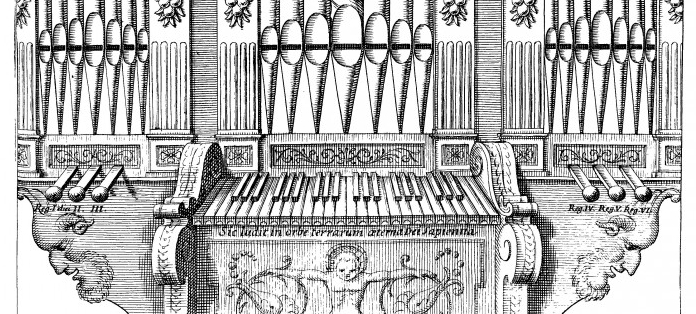
\includegraphics[width=\linewidth]{Kircher-creation-keyboard}
\end{figure}
%}}}4

Cererols, then, could be presenting his hearers with an auditory symbol of this
impossible music.
By pointing out the imperfect artifice of the music itself, Cererols prompts
listeners to reflect on how the imperfect reflects God's perfection.
In the theological context of this Christmas villancico, the \quoted{newest
consonance} is, of course, Christ himself.
As in Gutiérrez de Padilla's villancico, this piece makes Christ the
\term{Verbum infans}, the Word made flesh as an unspeaking infant.
The \quoted{sighs} of the baby, referred to several times in the text, are the
\quoted{new song} that becomes the cantus firmus of a renewed creation.
Through Cererols's interplay of motives and styles, listeners can actually hear
the music of human and divine emerging over the course of the piece,
culminating in the evocation of a motet based on motive B and ending with a
final flourish based on motive A.
Neither motive or style solely represents Christ's voice; rather the theme is
the paradoxical mixture of divine and human in the Incarnation.

\index{paradox}
\index{Incarnation}
\index{\emph{Verbum infans}}
\index{Gutiérrez de Padilla, Juan}

It is even possible to hear the whole estribillo as following a similar
Quintilian rhetorical structure to that of contemporary organ praeludia.%
    \Autocite{Jacobson:BuxtehudeRhetoric}
It opens with an attention-grabbing \term{exordium}, presents a central idea or
\term{propositio} (\term{la más nueva consonancia}), and then discusses the
idea through a series of statements, objections, and rebuttals (\term{narratio}
with \term{confutatio/confirmatio} pairs---the contrasts of modern and
contrapuntal styles), and closes with a rousing call to action
(\term{peroratio}, the final phrase).
If the villancico is an oration, then its main subject is Christ as \term{Verbum
infans}.
In Christ God entered the world of change and decay \quoted{to bring consonance
to the clay}.
Christ, particularly in his Passion and then in the Eucharist, was both
consonance and dissonance, old and new, material and spiritual.

\index{rhetoric}
%}}}2
%}}}1

%{{{1 sec: genealogy
\section{Genealogies of Heavenly Music}

If this villancico by Cererols were the only one of its kind it might register
as an interesting footnote, but in fact this setting is part of the
best-attested family of villancicos yet discovered from the seventeenth century.
Evidence survives for eight other settings of this poem in several variant
textual families, from its first known appearance in Madrid at Christmas 1651
through performances in Toledo, Zaragoza, Seville, and a fragmentary setting
from a convent in Ecuador (\tabref{tab:suspended-sources}).
The composers of most of these settings were closely linked in a web of personal
affiliations.
Their choice to set a text previously set by a teacher, colleague, or rival
enabled them to situate themselves within a tradition of both composition and
theology.

\index{affiliation}
\index{networks}
\index{villancico!families|(}
\index{villancico!circulation|(}

%{{{4 table Suspended sources
\begin{table}
    \caption{Sources of \wtitle{Ha de los coros/Suspended cielos}: Poetry
    imprints and musical settings}
    \label{tab:suspended-sources}
    \includefloat{suspended-sources}
\end{table}
%}}}4

Similar to the textual family of Gutiérrez de Padilla's \wtitle{Voces}, the
earliest surviving versions of the \wtitle{Suspended, cielos} family suggest an
earlier common source, as yet undiscovered.%
\begin{Footnote}
    Gutiérrez de Padilla quite likely was familiar with this villancico as
    well, although no setting by him survives, since the 1651 Madrid imprint
    in which the text first appeared includes another text that the Puebla
    chapelmaster did set in 1653, \wtitle{Alto zagales de todo el ejido} (see
    \musref{mus:Padilla-Alto_zagales-chaz}).
\end{Footnote}
The \wtitle{Suspended, cielos} estribillo is the most consistent element across
the versions.
The earliest imprint from the Royal Chapel in Madrid 1651 lacks a line that,
despite other variations, is present in six of the other sources, and which
makes metrical and poetic sense.
An earlier source, with this missing line, would have the form shown in
\tabref{tab:suspended-original}.
All of the versions except the highly abridged S10 are framed by eleven-syllable
lines (\poemlines{1, 16}).
After the \term{exordium}-like opening line, there follow three quatrains, each
in an \term{abbc} rhyme scheme where the final lines of all three stanzas rhyme
with each other.
The estribillo's conclusion is sealed with the \term{lira}-like three lines with
a 7--7--11 pattern of syllable counts.
The main variants constitute omitting one or two of these quatrains or portions
of them.
The Cererols version omits the second.
The compositors of these texts, whether chapelmasters or others, may have had
several motives for revision.
For one, omitting the references to Matins \quoted{tonight} and the stable
served to make the piece more adaptable for general purposes. 
Additionally, as polyphonic settings of villancicos became more complex and
included longer sections there were practical advantages to shortening the
text.

\index{Gutiérrez de Padilla, Juan}
\index{Madrid!Royal Chapel}

%{{{4 table Suspended original
\begin{table}
    \caption{Reconstructed original text of \wtitle{Suspended, cielos}
    estribillo} 
    \label{tab:suspended-original}
    \includefloat{suspended-original}
\end{table}
%}}}4

The two earliest sources precede this section with a \term{romance} of notable
elegance, beginning \foreign{Ha de los coros del cielo}
(\poemref{poem:Ha_de_los_coros}).
These stanzas set the scene for the rest of the villancico and clarify its
central musical conceit.
They clearly address not Heaven (\term{el cielo Empyreo}) but the heavens, the
planetary spheres.
The fourth stanza goes beyond puns on musical terms to paint a dramatic moment
of performance.
The \quoted{sapphires}, scattered across the sky like notes on a \quoted{starry
notebook}, must \quoted{make a rest} at the sound of \quoted{the newest
consonance}.
As though looking up in wonder at this new music, higher even than them, the
astral musicians let their sheets of music fall closed.%
\begin{Footnote}
    This suggests another allusion to the Last Day, when \quoted{the skies will
    be rolled up like a scroll} (\scripture{Is 34:4; Rev 6:14}).
\end{Footnote}
Like the painting of the Monsterrat Escolania beneath the Black Virgin, the
musical terms here are specific to the performance practice of villancicos as
opposed to Latin-texted polyphony.
The spheres are singing from \foreign{cuadernos}---partbooks, not a
choirbook---made up of one or two folded sheets of paper (\foreign{hojas
dobladas}) gathered together in a folder (\foreign{cartapacio}).

\index{\emph{romance} poetry}
\index{Montserrat!Escolania}
\index{performers}

%{{{4 poem Ha de los coros
\begin{poemexample}
    \caption{\wtitle{Ha de los coros del cielo}, opening \term{romance} in
    \term{Suspended, cielos} tradition, earliest version (S1) (roman numerals
    are indications of different speakers in original source)}
    \label{poem:Ha_de_los_coros}
    \includefloat{Ha_de_los_coros}
\end{poemexample}
%}}}4

Based on the variants of this romance and the coplas we may group the
texts in two families and identify genealogical relationships
(\diaref{dia:suspended-tree}).
Family A starts with the romance, \wtitle{Ha de los coros del cielo},
followed by the estribillo, \wtitle{Suspended, cielos, vuestro dulce canto},
then several coplas.
S2 has a unique set of coplas; the others all start with \foreign{Las fugas del
primer hombre}.

%{{{4 diagram suspended tree
\begin{diagram}
    \caption{Genealogical relationships among sources in \wtitle{Suspended,
    cielos} family (S1, source listed in \tabref{tab:suspended-sources}; F1,
    hypothetical source \add{\foreign{fuente}})}
    \label{dia:suspended-tree}
    \includefloat{suspended-tree}
\end{diagram}
%}}}4

Family B descends from a recension by Manuel de León Marchante, who somewhat
simplified the earlier version.%
    \Autocite[139]{LeonMarchante:Obras1733}
Family B moves all or part of the romance to the coplas in various ways.
These texts share other variant readings that mark their descent from a common
source (\tabref{tab:suspended-variants-estribillo}, 
\ref{tab:suspended-variants-coplas}).
This change demonstrates a transition in the later seventeenth century away from
using introductory romance sections and toward beginning directly with
the estribillo.%
    \Autocite{Torrente:Estribillo}
In many of the same ways that \wtitle{Cantores de la capilla} simplified
\wtitle{Voces, las de la capilla} (\chapref{ch:padilla-voces}), León Marchante
reduces the complexity and ambiguity of the earlier versions at the expense of
some nuances of the theological and musical conceits.
He omits the most grammatically and poetically difficult copla of the 1651
source (\foreign{Qué mucho si a los despeños}) along with three others.
He changes the first word of \foreign{siglos de los astros} (centuries/ages of
the stars) to \foreign{signos} (signs). 
Where \foreign{siglos} (also used in \wtitle{Voces}) referred obliquely both to
time and planetary motion, \foreign{signos} is more clearly a musical term that
still has a planetary double meaning.
León Marchante also changes the last word of \foreign{En las pajas subtenido}
to \foreign{sustenido}, substituting a clear musical play on words (Christ
\quoted{sustained} on the bed of straw/Christ singing a \quoted{sharp}) for the
more arcane geometrical concept of a line that joins together two extremes of
an arc, as Christ joins together eternal and temporal.

\index{León Marchante, Manuel de}
\index{\emph{conceptismo}}

%{{{4 tables Suspended variants
\begin{table}
    \caption{Variants in the estribillo of \wtitle{Suspended, cielos}
    villancicos, compared with reconstructed original source
    (\tabref{tab:suspended-original})}
    \label{tab:suspended-variants-estribillo}
    \includefloat{suspended-variants-estribillo}
\end{table}

\begin{table}
    \caption{Variants in the romance and coplas of \wtitle{Suspended, cielos}
    villancicos} 
    \label{tab:suspended-variants-coplas}
    \includefloat{suspended-variants-coplas}
\end{table}
%}}}4

Sources 4--6 were all produced in a three-year period by composers (cited by
name in the imprints) who were all personally acquainted with each other and
regularly exchanged villancico texts.
León Marchante wrote or edited a large number of texts for Toledo Cathedral,
where they were set to music by chapelmaster Pedro de Ardanaz.
Ardanaz's correspondence with Miguel de Irízar, chapelmaster in Segovia and
fellow student of Tomás Miciezes the elder, reveals that villancico poems were
exchanged through a network that also included Diego de Cáseda, another fellow
pupil who was chapelmaster in Zaragoza.%
    \Autocites
    {Rodriguez:Networks}
    [302--311]{Cashner:PhD}
Ardanaz probably also shared the texts with another Miciezes alumnus, Alonso
Xuárez (Suárez) in Seville (S4).
After Xuárez's version at Seville Cathedral for Christmas 1680, S5 was performed
a year later at Seville's second most important church-music institution, the
church of San Salvador, in a closely related but abridged text with only five
coplas.
The composer was Miguel Mateo de Dallo y Lana.
S6 was sung twelve days later for Epiphany 1683 in Zaragoza in a setting by
Cáseda.

\index{Toledo Cathedral}
\index{Ardanaz, Pedro de}
\index{Irízar, Miguel de}
\index{Segovia Cathedral}
\index{Miciezes, Tomás (elder)}
\index{Cáseda, Diego de}
\index{Zaragoza}
\index{Xuárez, Alonso}
\index{Suárez, Alonso|see{Xuárez, Alonso}}
\index{Seville!Cathedral}
\index{Seville!San Salvador}
\index{Dallo y Lana, Miguel Mateo de}


The 1689 Royal Chapel version returns to the original source in a similar manner
to Gutíerrez de Padilla turning away from \wtitle{Cantores} back to
\wtitle{Voces}.
Some of the chapel musicians probably remembered the 1651 performance, and
their leader at that time, interim director Juan de Navas, likely had access to
the original parts and imprint in the archive.%
    \Autocite[\sv{Capilla Real}]{DMEH} 
The text is closer to family A but includes some of León Marchante's
revisions from family B.
The two musical manuscripts by Cererols belong in family A, even though they
lack the \term{romance}, because they do not have any of León Marchante's
alterations.
This suggests that this version of the text was arranged around 1660, before
León Marchante adapted it.

\index{Navas, Juan de}
\index{Madrid!Royal Chapel}

%{{{2 ecuador
This network extended to South America as well: Source 10 resides in the remote
parish archive of Ibarra, Ecuador, among a collection originally from the
Conceptionist convent there.
It is a fragment of an anonymous eleven-voice setting, in three choirs, based on
a variant of this textual tradition, with only the third-chorus voices of the
estribillo.
The music may have been composed by one of the chapelmasters of Quito Cathedral
and adapted by the convent sisters for their own use.%
\begin{Footnote}
    Grateful acknowledgments to Cesar Favila for allowing me to view a scan of
    this source.
%    XXX source, info, names
\end{Footnote}
The manuscripts demonstrate that the piece was frequently performed and
readapted for different occasions.
The Tiple and Tenor parts bear the names of performers, \quoted{Sra. S. Martin}
and \quoted{Sra. S. Seçilia} respectively.
There is a second copy of the Alto part, copied in a different hand, with the
indication for dulzaina, a double-reed instrument.

\index{Ibarra, Ecuador!Conceptionist convent}
\index{villancico!performance practice}
\index{convent music}
\index{\emph{dulzaina}}

The text, as far as can be determined, has been made much more general so that
it could be used for almost any occasion (\poemref{poem:Suspended-Ecuador}).
Additional lyrics have been added in a different hand above the first line of
lyric text.
The text still mentions \foreign{planetas} but retains none of the themes of the
other sources.
Going farther than the variant Cererols manuscript (which changed \foreign{niño}
to \foreign{hombre} for a Eucharistic purpose), the compositor has changed
\foreign{niño} to \foreign{santo} (saint), allowing use for general sanctoral
devotion.
Some of the tropes continue to develop the earlier tradition.
The music depicts \quoted{stopping} and \quoted{listening} with halting
entrances set apart with rests, probably echoes of the other choruses
(\musref{mus:Suspended-Ecuador-1}, \ref{mus:Suspended-Ecuador-2}).
Like Cererols, this composer uses plainchant-like stepwise lines on \foreign{el
canto llano}.
On the other hand, the piece emphasizes \quoted{faith and devotion} over
cosmology, symbolism, and Neoplatonic contemplation.
This shift may be representative of a broader change in orientation away from
speculative and symbolic thinking and toward a more feeling-based personal
piety around the turn of the eighteenth century.

\index{villancico!liturgical function!sanctoral devotion}
\index{villancico!liturgical function!general-purpose}


%{{{4 poem and music, Suspended Ecuador
\begin{poemexample}
    \caption{\wtitle{Suspended vuestro canto}: Ecuador version of
    \wtitle{Suspended, cielos} (S10), extant text (added alternative texts
    shown in italics)}
    \label{poem:Suspended-Ecuador}
    \includefloat{Suspended-Ecuador}
\end{poemexample}

\begin{musicexample}
    \caption{\wtitle{Suspended vuestro canto} (Conceptionist Convent of
    Ibarra, Ecuador), surviving music, excerpt from beginning}
    \label{mus:Suspended-Ecuador-1}
    \includefloat{Suspended-Ecuador-1}
\end{musicexample}

\begin{musicexample}
    \caption{\wtitle{Suspended vuestro canto} (Ecuador), surviving music,
    excerpt from end}
    \label{mus:Suspended-Ecuador-2}
    \includefloat{Suspended-Ecuador-2}
\end{musicexample}
%}}}4

\index{villancico!families|)}
\index{villancico!circulation|)}
%}}}2
%}}}1

%{{{1 sec: conclusion
\section{The Problem of Perfection}

The family of \wtitle{Suspended, cielos} villancicos manifests a widespread
cultural fascination with heavenly music, and with the use of music to
represent itself.
The genealogy of these pieces, passing from hand to hand among interrelated
musicians, strengthens the argument that the metamusical villancico subgenre did
function as a favored way for these composers to prove their craftsmanship and
establish a place in the musical community.
The prevalence of a text so heavily dependent on Ptolemaic and
Neoplatonic-Boethian musical cosmology challenges Hollander's hypothesis of
secularization during the seventeenth century, at least for Catholic Spain.
At the same time, the Cererols setting, with its ambiguous symbolic use of
dissonance and contrasting musical styles, does suggest a certain anxiety about
the relation of earthly and heavenly music that seems distinct to this period.

\index{Hollander, John}
\index{secularization}
\index{Boethius}
\index{Neoplatonism}

This piece reveals a latent theological problem within musical thought and
practice in the early modern period: to what degree does the order of nature
reflect the perfection of God?
Is dissonance a necessary element of beautiful music, or is it a sign that
something is wrong with the system from its root?  
Does earthly music reflect the divine or express the human?
The development of the \term{Suspended, cielos} tradition, and the related
pieces studied in the other chapters, suggests that there was a gradual shift in
the function of Spanish villancicos about music from reflecting divine
perfection toward expressing human affects, away from emphasizing how worldly
music is like heavenly music and toward stressing its imperfections and
difference from higher forms.
This piece by Cererols stands at a midpoint where dissonance may function as a
symbol through which listeners may contemplate the imperfection and sin of the
fallen world; and as an ironic or paradoxical symbol that urges them to imagine
a higher form of music. 
At the same time dissonance is beginning to serve a positive aesthetic purpose
to elicit an affective response from listeners.
Later composers, as we will see, pushed the artifice even farther, going to
more extravagant ends to demonstrate the untunefulness and imperfection of
earthly music.

\index{counterpoint, symbolism}
\index{paradox}
\index{perfection}
\index{sin}

The adaptations of this text for other purposes (the Eucharistic Cererols
variant; the two alternate texts of the Ecuador manuscript) demonstrate the
appeal that this poetic conceit offered, but also suggest that as the century
progressed people began to see it as simply an attractive poetic conceit,
missing the intricate theological complexity of the earlier sources.
The eloquent exposition of Neoplatonic musical theology in the poetry imprints
and the Cererols setting is watered down in the Ecuador manuscript to a series
of vague conventions.
This fits with Hollander's thesis of increasing conventionalism in poetry on
music, but it does not corroborate his secularization theory.
Though the Ecuador text does not depend on the details of any particular
cosmology, that does not mean the authors or performers had ceased to believe in
the old system.
Besides, from only the third-chorus parts it is impossible to guess the full
content of the villancico text.  And even if the musical theology of the Ecuador
setting is relatively vague compared to the rest of the tradition, the original
piece still calls for no fewer than eleven voices to sing out an exhortation to
the planets.
The complicated conceits of this poetic tradition as seen in the earliest
sources may have fallen out of fashion, but the fundamental theological
framework underlying this poetic tradition still continued to provide meaning.
While Isaac Newton's new physics would soon illuminate the real structure of
the solar system, in the years just after the publication of the
\wtitle{Principia mathematica}, there were four separate performances of a
\wtitle{Suspended, cielos} villancico in the Spanish Empire, where the old
earth-centered worldview blazed its brightest just before sunset.

\index{Cererols, Joan|)}
\index{Montserrat!Abadia|)}
\index{Newton, Isaac}
\index{science}

%}}}1

\endinput

